

\documentclass[25pt,a0paper, portrait]{tikzposter}
\usepackage[utf8]{inputenc}
\usepackage{xcolor}
\usepackage{graphicx,mwe}
\usepackage{filecontents}
\usepackage{lipsum}
\usepackage{tikz}
\usepackage{multicol}
\usepackage{adjustbox}
\usepackage{blindtext}
\usepackage{comment}


 \makeatletter
\def\TP@titlegraphictotitledistance{-6cm}
\settitle{ \centering \vbox{
		\@titlegraphic \\ [\TP@titlegraphictotitledistance] 
		\centering
		\color{titlefgcolor} 
		{\bfseries \Huge \sc \@title \par}
		\vspace*{1em}
		{\huge \@author \par}
}}
\makeatother

\setlength{\columnsep}{2cm}
 
\title{Face Recognition using Portenta H7}
\author{Vatsal Mahajan, Manoj Selvaraju \& Vijay Singh}
\titlegraphic{
	%\vspace*{-2cm} % Adjust vertical spacing if needed
	\hspace*{-64cm} % Adjust horizontal spacing to move it to the left
	
\includegraphics[height=6.5cm]{images/logo_hs_technik}
}
 
\usetheme{Desert}
 
\begin{document}
	
	\maketitle
	
	\begin{columns} 
		
		\column{0.6}
		
		\colorlet{blocktitlebgcolor}{blue}
		\block{Topic Description}
		{
			
			The goal of our project is to develop a face recognition-based access control system using machine learning. The project involves capturing facial images using the Vision Shield, preprocessing the data, training a CNN-based model with Edge Impulse and optimizing it for real-time inference on the Arduino Portenta H7. The system includes profile management functionalities such as adding and deleting users to enhance security and flexibility.
			
		}
		
		\colorlet{blocktitlebgcolor}{blue}
		\block{Description of our Application}
		{
			\textbf{Dataset:}
			Three distinct images representing Person1, Person2, and Person3.
			
			\subsection*{Features:}
			Facial features which are used to distinguish between individuals.
			
			\subsection*{Image Type:}
			The images used are grayscale, simplifying the model’s task of feature extraction.
			
			\subsection*{Model:}
			A CNN-based MobileNetV2 model is used, capable of distinguishing between different people for accurate classification.
			
			\subsection*{Hardware:}
			The system uses an Arduino Portenta H7, Vision Shield and a USB-C cable to facilitate the recognition process.
			
			\subsection*{Software:}
			Arduino IDE, Edge Impulse CLI, Python and Node.js for implementing and deploying the model.
			
			
		}
		
		\colorlet{blocktitlebgcolor}{blue}
		\block{Challenges}
		{
			
	\subsection*{Optimised Image Resolution:}  
	Building the model using higher resolutions, such as QVGA (320x240) or lower than QQVGA (128x96) from the Vision Shield camera, led to significant overfitting issues.  

	\subsection*{Profile Management:}  
	Attempted to add new profiles and retrain the model in Edge Impulse Studio using API keys, but faced challenges with API integration.  

	\subsection*{Model Accuracy vs. Size:}  
	Keeping the model lightweight for deployment while maintaining high accuracy was a challenge.  

	\subsection*{Lighting and Environmental Conditions:}  
	Struggled with varying lighting conditions (e.g., too bright or too dark) and environmental factors (e.g., glare or shadows).  

			
		}
		
		
		
		\colorlet{blocktitlebgcolor}{blue}
		\block{Solution}
		{
	\subsection*{Optimised Image Resolution:}
	Choose QQVGA (160x120) resolution to balance image quality, which reduces overfitting during model training while ensuring accurate recognition.

	\subsection*{Profile Management:}
	Manually update the dataset and retrain the model in Edge Impulse Studio \cite{edgeimpulse:2025}, prioritizing accuracy over automation.

	\subsection*{Model Accuracy vs. Size:}
	Apply model quantization (int8) \cite{mathworksint8quantization:2025} techniques to reduce model size without compromising accuracy.

	\subsection*{Lighting and Environmental Conditions:}
	Ensure optimal hardware placement in environments with balanced lighting to minimize the effects of glare, shadows, and extreme brightness.

			
		}
		
		
		
		\column{0.4}

		\colorlet{blocktitlebgcolor}{blue}	
		\block{Model Evaluation Metrics}
		{
		\section*{Performance Metrics}			
		\subsection*{Accuracy: 
			85.20\% \newline}
	
	
		\subsection*{Confusion Matrix}
		\textbf{<F1 Score> } Harmonic mean of precision and recall.
		
		\begin{tikzfigure}
		
			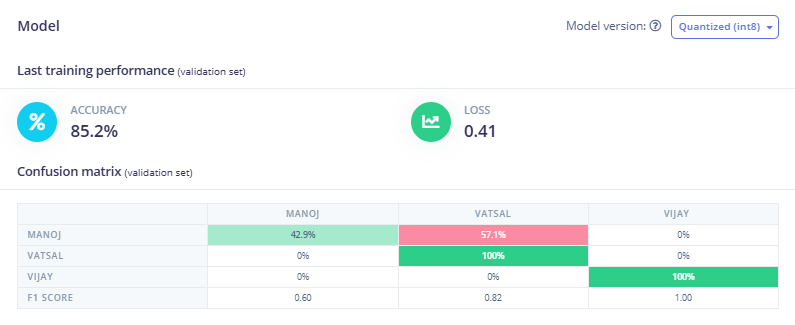
\includegraphics[width=\linewidth]{images/Interpretation}
		
		\end{tikzfigure}
	
}
		\colorlet{blocktitlebgcolor}{blue}
		\block{Results}
		{
			\begin{itemize}
				\item Once the model is successfully uploaded to the device, inference is triggered using the Edge Impulse command. 
				\item This process generates local visualizations on the host machine, providing a graphical user interface (GUI) for face recognition, as illustrated below.
			\end{itemize}

			\begin{tikzfigure}
				
				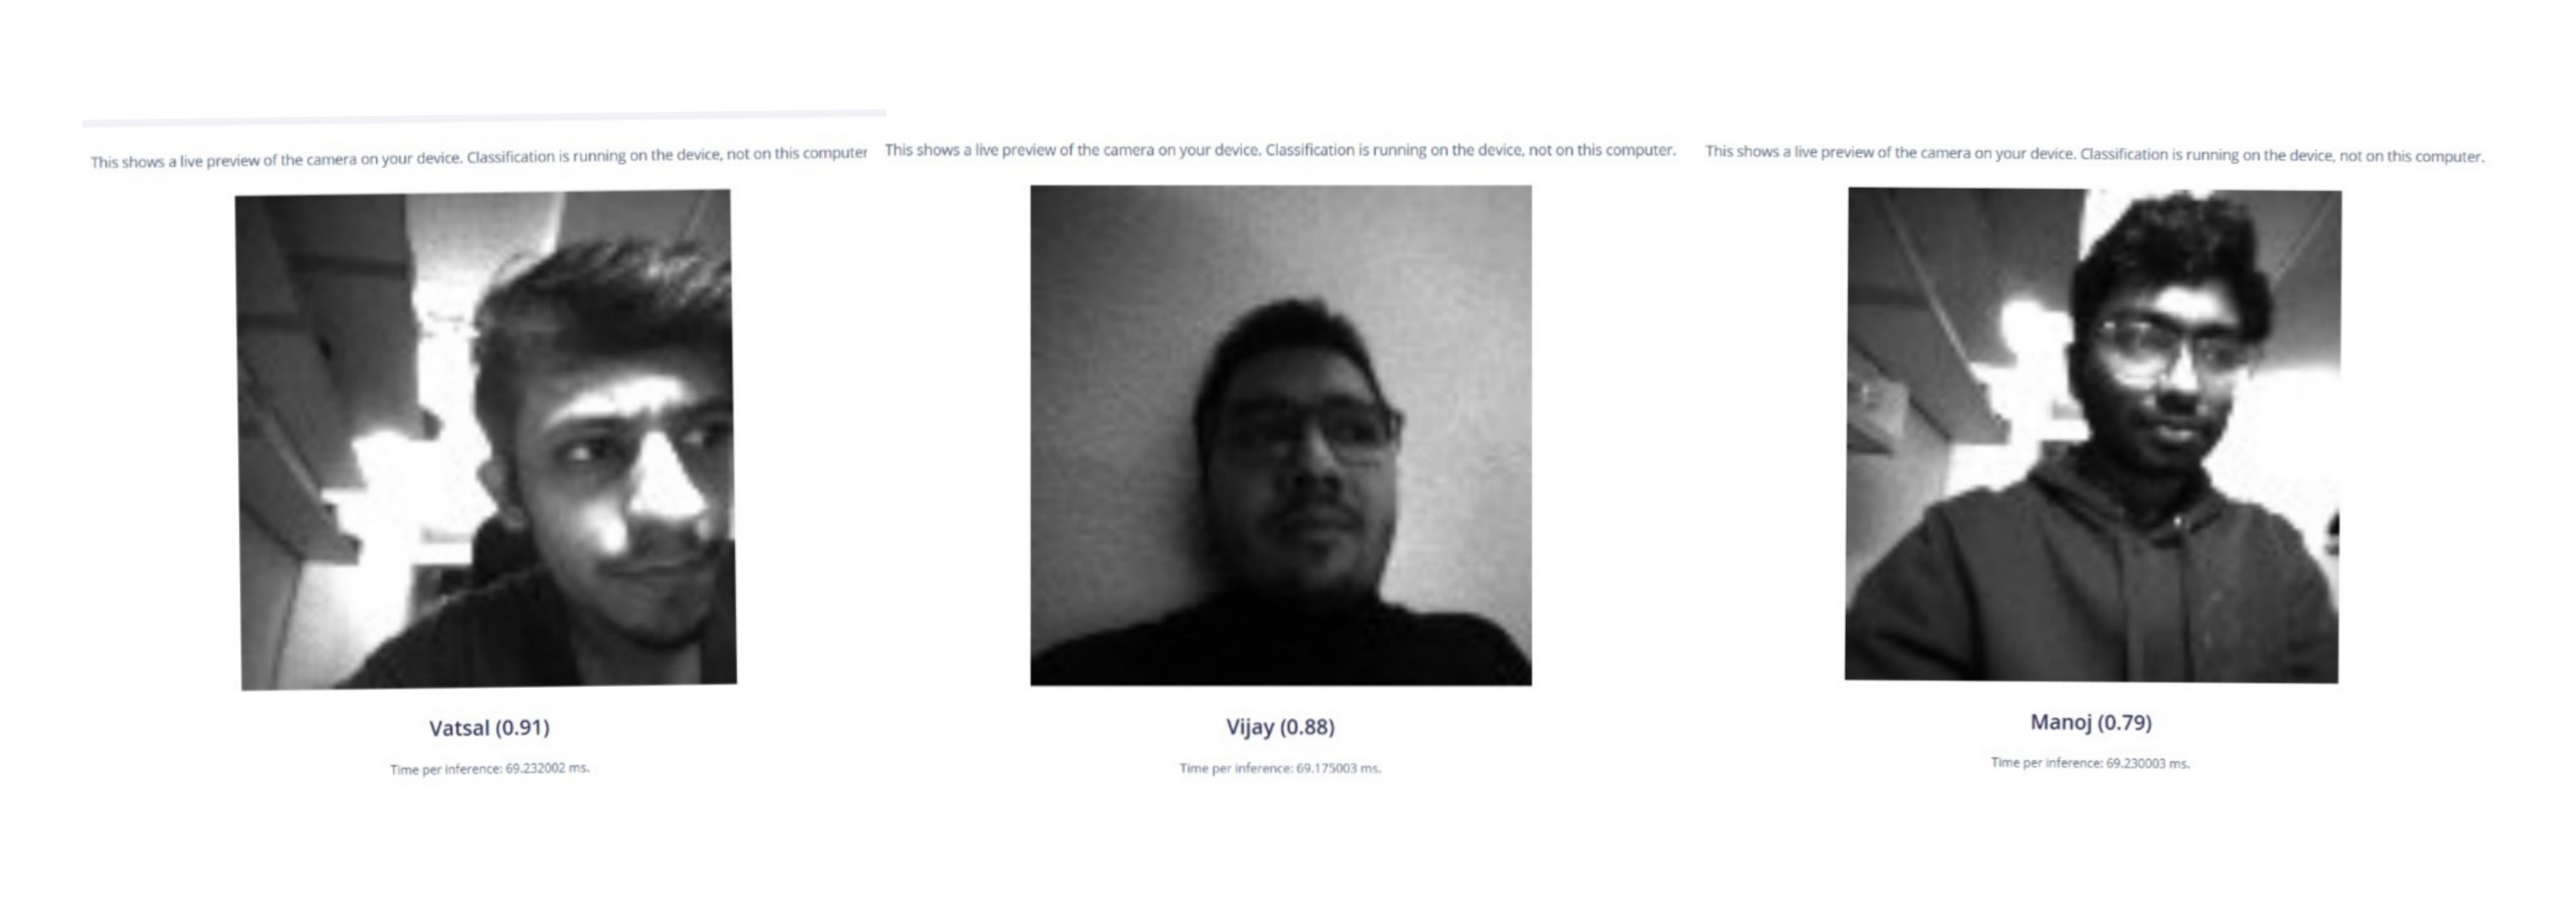
\includegraphics[width=\linewidth]{images/faceresult}
				
			\end{tikzfigure}
			\subsection*{Recognised Facesets:} 
			\begin{itemize}
				\item Vatsal (0.91)
				\item Vijay (0.88)
				\item Manoj (0.79)
			\end{itemize}	
			
			
		}
		
		\colorlet{blocktitlebgcolor}{blue}
		\block{Conclusion}
		{
	\begin{itemize}
		\item Developed a face recognition system for access control using the Portenta H7 and Vision Shield.
		\item The optimized model achieved an accuracy of 85.2\% during testing, effectively recognizing faces across all trained profiles.
		\item The system successfully handled varied lighting conditions with the balanced dataset.
		\item Supported profile updates and deletions, ensuring flexibility and efficient access control.
	\end{itemize}

		}
		
		
		
		\colorlet{blocktitlebgcolor}{blue}
		\block{References}
		{			
			\small
			\bibliographystyle{plain}
			
			\bibliography{Documents/MyLiterature.bib}
			
		}
		
		
	\end{columns}
	
\end{document}